\chapter{Resultados} % (fold)
\label{cha:resultados}
% http://pypi-ranking.info/alltime
% http://popcon.ubuntu.com/
% http://popcon.debian.com/

\begin{table}[htbp]
\caption{Comparação de resultados}
\begin{tabular}{|c|l|c|c|c|p{2cm}|}
\hline
\multicolumn{ 2}{|c|}{\textbf{Pacote}} & \textbf{Apt-Cache} & \textbf{Exact Match} & \textbf{Levenshtein} & \textbf{Smith-Waterman} \\ \hline\hline
\multicolumn{ 1}{|c|}{} & \textit{[position]} &  &  &  &  \\ \cline{ 2- 6}
\multicolumn{ 1}{|c|}{\textbf{dpkg}} & \textit{[len]} &  &  &  &  \\ \cline{ 2- 6}
\multicolumn{ 1}{|c|}{} & \textit{[time]} &  &  &  &  \\ \hline
\multicolumn{ 1}{|c|}{} & \textit{[position]} &  &  &  &  \\ \cline{ 2- 6}
\multicolumn{ 1}{|c|}{\textbf{debianutils}} & \textit{[len]} &  &  &  &  \\ \cline{ 2- 6}
\multicolumn{ 1}{|c|}{} & \textit{[time]} &  &  &  &  \\ \hline
\multicolumn{ 1}{|c|}{} & \textit{[position]} &  &  &  &  \\ \cline{ 2- 6}
\multicolumn{ 1}{|c|}{\textbf{coreutils}} & \textit{[len]} &  &  &  &  \\ \cline{ 2- 6}
\multicolumn{ 1}{|c|}{} & \textit{[time]} &  &  &  &  \\ \hline
\multicolumn{ 1}{|c|}{} & \textit{[position]} &  &  &  &  \\ \cline{ 2- 6}
\multicolumn{ 1}{|c|}{\textbf{dash}} & \textit{[len]} &  &  &  &  \\ \cline{ 2- 6}
\multicolumn{ 1}{|c|}{} & \textit{[time]} &  &  &  &  \\ \hline
\multicolumn{ 1}{|c|}{} & \textit{[position]} &  &  &  &  \\ \cline{ 2- 6}
\multicolumn{ 1}{|c|}{\textbf{perl-base}} & \textit{[len]} &  &  &  &  \\ \cline{ 2- 6}
\multicolumn{ 1}{|c|}{} & \textit{[time]} &  &  &  &  \\ \hline
\end{tabular}
\subcaption{Fonte: \href{http://popcon.ubuntu.com/}{Popcorn-Ubuntu}\protect\footnotemark}
\label{tab:comparacao}
\end{table}
\footnotetext{\label{tab:comparacao_footnote}Ordenado pelo número de pessoas que usam o pacote regularmente}

\begin{figure}[h]
  \centering
	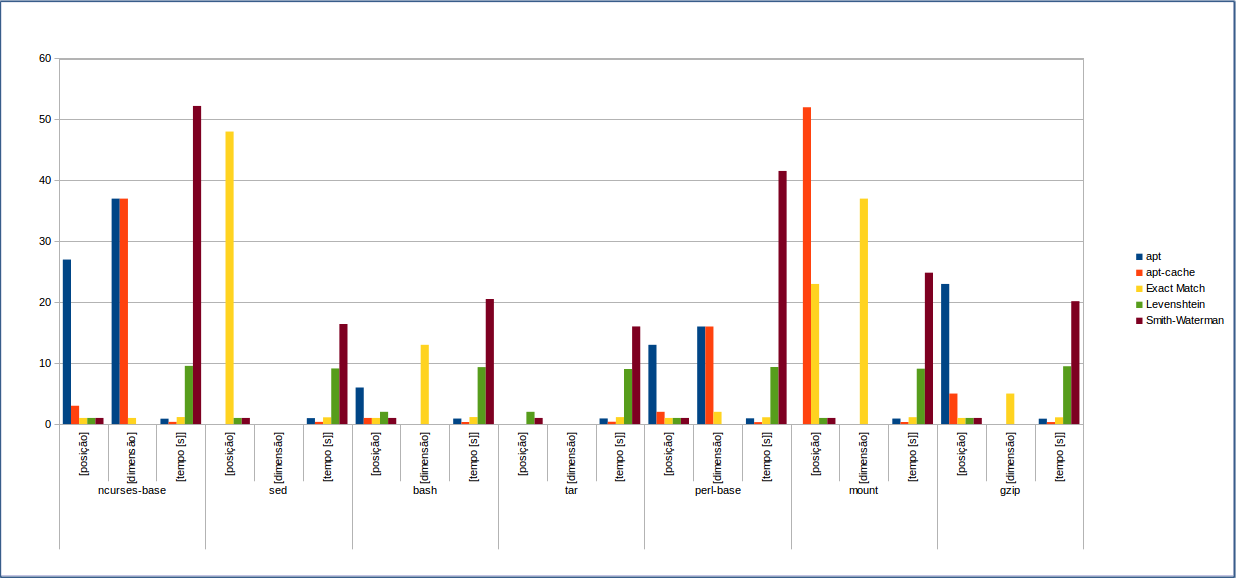
\includegraphics[width=0.8\textwidth]{figuras/grafico}
  \caption{Exemplo de amostra}
  \label{fig:figuras_grafico}
\end{figure}

\lipsum[1]